%----------------------------------------------------------------------------------------
%	PACKAGES AND DOCUMENT CONFIGURATIONS
%----------------------------------------------------------------------------------------

\documentclass{article}


\usepackage{graphicx} % Required for the inclusion of images
\graphicspath{{figures/}}
\usepackage{subfigure} % Required for the inclusion of images
\usepackage{natbib} % Required to change bibliography style to APA
\usepackage{amsmath} % Required for some math elements 
\usepackage{listings}
\usepackage{xcolor}
\usepackage{fontspec}
\usepackage{ctex}
\usepackage{geometry}
\geometry{a4paper,scale=0.8}
\renewcommand{\contentsname}{\centerline{目录}}
\setmonofont{Consolas}
\lstset{
basicstyle=\ttfamily\footnotesize,%
escapeinside=``,%
keywordstyle=\color{black},%\bfseries, \underbar,%
identifierstyle={},%
tabsize=4,
commentstyle=\color{blue},%
stringstyle=\ttfamily,%
%labelstyle=\tiny,%
extendedchars=false,%
linewidth=\textwidth,%
numbers=left,%
numberstyle=\tiny \color{blue},%
frame=trbl%
}
%点列
%\begin{itemize}
%\item[$\bullet$]Get familiar with Y86 assembly language.
%\end{itemize}

%小标题
%\begin{center}
%{\ttfamily rsum.ys}
%\end{center}
%代码
%\begin{lstlisting}[language={[ANSI]C}]
%\end{lstlisting}
%点列和浮动体图表和ref
%\begin{itemize}
%\item[$\bullet$]{\ttfamily sum.ys} (Figure \ref{Part A: sum.ys})\\
%\end{itemize}
%\begin{figure}[htbp]%figure浮动体环境 [htbp]指定位置
%		\centering%居中排版
%		\includegraphics{A_sum}
%		\caption{Part A  {\ttfamily sum.ys}} \label{Part A: sum.ys}%标题 自动编号 label标签
%\end{figure}


%\usepackage{times} % Uncomment to use the Times New Roman font

%----------------------------------------------------------------------------------------
%	DOCUMENT INFORMATION
%----------------------------------------------------------------------------------------

\title{\textbf{操作系统课程设计Project 1\\Introduction to Linux Kernel  Modules}} % Title

\author{姓名: 郭倩昀  
\\班级: F1903303  
\\学号: 519021910095  
\\Email: guoqianyun@sjtu.edu.cn} % Author name and email
\date{\today} % Date for the report
\begin{document}
\maketitle % Insert the title, author and date
\tableofcontents
\newpage
\section{Introduction to Linux Kernel  Modules}
\subsection{实验内容与目标}
\begin{itemize}
\item[$\bullet$]熟悉内核模块
\item[$\bullet$]内核模块的创建、加载与卸载
\item[$\bullet$]设计内核模块,给/proc文件系统创建新条目
\end{itemize}

\subsection{实验过程及步骤}
\begin{itemize}
%\begin{ttfamily}
\item[$\bullet$]配置环境\\
本次project需要在Linux系统的虚拟机环境下完成,因此首先安装虚拟机virtualbox,并安装Ubuntu系统,鉴于版本兼容原因我选择了安装ubuntu-16.04.7-desktop-amd64版本,进行了部分必要的软件更新操作。
\item[$\bullet$]熟悉内核模块\\
在ubuntu系统中输入lsmod可以查看目前系统加载的所有内核模块,包括module name, size, used by等信息。\\
分析源代码simple.c文件熟悉基本内核模块的组成部分,熟悉模块入口点和模块出口点函数。\\
simple.c文件需要经过Makefile编译,命令行语句输入make即可完成。
\item[$\bullet$]修改内核模块\\
根据project要求,为了在simple\_init()中输出GOLDEN\_RATIO\_PRIME、jifffies和HZ,在函数中添加语句:\\
	printk(KERN\_INFO "  GOLDEN\_RATIO\_PRIME = \%lu$\backslash$n", GOLDEN\_RATIO\_PRIME);\\
	printk(KERN\_INFO "  jiffies = \%lu$\backslash$n",jiffies);\\
	printk(KERN\_INFO "  HZ = \%lu$\backslash$n",HZ);\\
为了在simple\_exit()函数中输出3300和24的最大公约数以及jiffiles数值,在函数中添加语句:\\
	printk(KERN\_INFO "  gcd = \%lu$\backslash$n",gcd(3300,24));\\
	printk(KERN\_INFO "  jiffies = \%lu$\backslash$n",jiffies);\\
修改后的代码见实验代码部分。
\item[$\bullet$]加载和卸载内核模块\\
首先可以通过命令 sudo dmesg -C来清空内核日志缓冲区,其中sudo作为指令前缀可以获取管理员权限,但此时需要输入密码,或者可以登录终端的时候输入sudo su root来切换到管理员权限。\\
输入sudo insmod simple.ko可以加载内核模块simple,输入dmesg可以查看到内核日志信息“Loading Module simple”以及project要求在simple\_init()输出的任务,表示内核模块加载成功;输入sudo rmmod simple可以卸载内核模块,再次输入dmesg可以查看到内核日志信息“Removing Module simple”以及project要求在simple\_exit()输出的任务,表示内核模块卸载成功。\\
实验测试结果见实验测试部分。
\item[$\bullet$]熟悉/proc文件系统内核模块\\
以教材中源代码hello.c为例熟悉/proc文件系统内核模块的基本组成部分和对应功能。hello模块加载后输入命令cat /proc/hello会输出Hello World。
\item[$\bullet$]设计/proc文件系统内核模块jiffies和seconds\\
模仿hello模块设计jiffies模块和seconds模块,增加相应的头文件,在proc\_read函数中修改输出为相应的jiffies和seconds(根据proc\_init和proc\_read两次读取的jiffies计算得出) 。测试时首先用Makefile编译模块的时候注意需要将文件名称修改为编译对象名称。\\
测试的时候内核加载和卸载同之前的simple模块一样,加载了模块后输入命令cat /proc/jiffies以及cat /proc/seconds会输出相应的任务结果。具体代码和测试结果见实验代码和实验测试部分。
%\end{ttfamily}
\end{itemize}
\subsection{实验代码}
\begin{center}
{\ttfamily simple.c}
\end{center}
\begin{lstlisting}[language={[ANSI]C}]
#include <linux/init.h>
#include <linux/module.h>
#include <linux/kernel.h>
#include <linux/gcd.h>
#include <linux/hash.h>
#include <asm/param.h>
#include <linux/jiffies.h>

/* This function is called when the module is loaded. */
int simple_init(void)
{
       printk(KERN_INFO "Loading Module simple\n");
	printk(KERN_INFO "  GOLDEN_RATIO_PRIME = %lu\n", GOLDEN_RATIO_PRIME);
	printk(KERN_INFO "  jiffies = %lu\n",jiffies);
	printk(KERN_INFO "  HZ = %lu\n",HZ);
       return 0;
}

/* This function is called when the module is removed. */
void simple_exit(void) {
	printk(KERN_INFO "Removing Module simple\n");
	printk(KERN_INFO "  gcd = %lu\n",gcd(3300,24));
        printk(KERN_INFO "  jiffies = %lu\n",jiffies);

}

/* Macros for registering module entry and exit points. */
module_init( simple_init );
module_exit( simple_exit );

MODULE_LICENSE("GPL");
MODULE_DESCRIPTION("Simple Module");
MODULE_AUTHOR("GQY");
\end{lstlisting}
\begin{center}
{\ttfamily jiffies.c}
\end{center}
\begin{lstlisting}[language={[ANSI]C}]
#include <linux/init.h>
#include <linux/kernel.h>
#include <linux/module.h>
#include <linux/proc_fs.h>
#include <linux/jiffies.h>
#include <linux/sched.h>
#include <linux/uaccess.h>

#define BUFFER_SIZE 128
#define PROC_NAME "jiffies"

ssize_t proc_read(struct file *file,char __user *usr_buf,size_t count,loff_t *pos);

static struct file_operations proc_ops ={
.owner = THIS_MODULE, 
.read = proc_read,  
};

/* This function is called when the module is loaded. */
int proc_init(void)
{
    proc_create(PROC_NAME,0666,NULL,&proc_ops); 
    printk(KERN_INFO "/proc/%s created\n", PROC_NAME);
    return 0;
}

void proc_exit(void)
{
    remove_proc_entry(PROC_NAME,NULL);  
    printk( KERN_INFO "/proc/%s removed\n", PROC_NAME);
}


ssize_t proc_read(struct file *file, char __user *usr_buf, size_t count, loff_t *pos)
{
    int rv=0;  
    char buffer[BUFFER_SIZE];  
    static int completed=0;
    if (completed){
      completed=0;
      return 0;
    }
    completed=1;
     
    rv=sprintf(buffer, "Now the jiffies value is %lu\n", jiffies); 
    copy_to_user(usr_buf,buffer,rv);
    return rv;
}
module_init(proc_init);
module_exit(proc_exit);

MODULE_LICENSE("GPL");
MODULE_DESCRIPTION("Display the jiffies value"); 
MODULE_AUTHOR("GQY"); 

\end{lstlisting}
\begin{center}
{\ttfamily seconds.c}
\end{center}
\begin{lstlisting}[language={[ANSI]C}]
#include <linux/init.h>
#include <linux/kernel.h>
#include <linux/module.h>
#include <linux/proc_fs.h>
#include <linux/sched.h>
#include <linux/uaccess.h>
#include <linux/jiffies.h>/* jiffies*/
#include <asm/param.h> /* HZ*/

#define BUFFER_SIZE 128
#define PROC_NAME "seconds"


unsigned long int volatile jiffies1,jiffies2;
const int hz=HZ;

ssize_t proc_read(struct file *file,char __user *usr_buf,size_t count,loff_t *pos);


static struct file_operations proc_ops ={
.owner = THIS_MODULE,
.read = proc_read,   
};

/* when the module loaded*/
int proc_init(void)
{
    proc_create(PROC_NAME,0666,NULL,&proc_ops);
    jiffies1 = jiffies;  
    printk(KERN_INFO "/proc/%s created\n", PROC_NAME);
    return 0;
}

void proc_exit(void)
{
    remove_proc_entry(PROC_NAME,NULL);
    printk( KERN_INFO "/proc/%s removed\n", PROC_NAME);
}

/*Implemention of proc_read*/
ssize_t proc_read(struct file *file, char __user *usr_buf, size_t count, loff_t *pos)
{
	jiffies2 = jiffies;  
    int rv=0;
    char buffer[BUFFER_SIZE];
    static int completed=0;
    if (completed){
      completed=0;
      return 0; 
    }
    completed=1;
    rv=sprintf(buffer, "The running time is %d s\n", ((jiffies2-jiffies1)/hz));
 
    copy_to_user(usr_buf,buffer,rv);
    return rv;
}
module_init(proc_init);
module_exit(proc_exit);

MODULE_LICENSE("GPL");
MODULE_DESCRIPTION("Show the program execution time");
MODULE_AUTHOR("GQY");

\end{lstlisting}
\subsection{实验测试}
\begin{itemize}
\item[$\bullet$]测试simple模块(图 \ref{测试simple模块})
\end{itemize}
\begin{figure}[htbp]
		\centering
		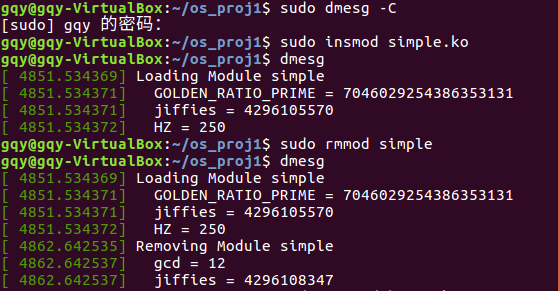
\includegraphics{simple}
		\caption{测试simple模块} \label{测试simple模块}
\end{figure}
\begin{itemize}
\item[$\bullet$]测试hello模块(图 \ref{测试hello模块})
\end{itemize}
\begin{figure}[htbp]
		\centering
		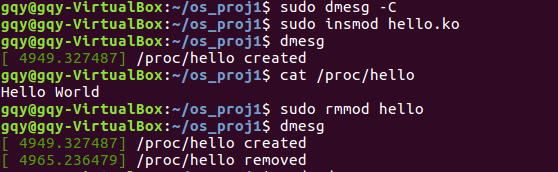
\includegraphics{hello}
		\caption{测试hello模块} \label{测试hello模块}
\end{figure}
\begin{itemize}
\item[$\bullet$]测试jiffies模块(图 \ref{测试jiffies模块})
\end{itemize}
\begin{figure}[htbp]
		\centering
		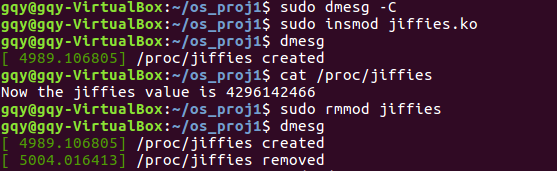
\includegraphics{jiffies}
		\caption{测试jiffies模块} \label{测试jiffies模块}
\end{figure}
\begin{itemize}
\item[$\bullet$]测试seconds模块(图 \ref{测试seconds模块})
\end{itemize}
\begin{figure}[htbp]
		\centering
		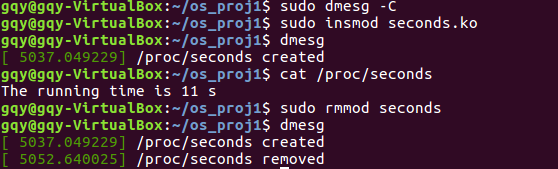
\includegraphics{seconds}
		\caption{测试seconds模块} \label{测试seconds模块}
\end{figure}
\section{Conclusion}
\subsection{问题与解决方案}
本次project的内容基本上比较简单,一步步按照书上的指示就可以顺利完成。不过实验过程中的还是出现了一些小问题,首先就是在编译内核模块的时候,因为课本给予的示例是给予旧版本的内核,但由于ubuntu系统版本以及内核版本的变化,部分函数(如proc\_create)的定义也有了变化,同时有一些头文件的已经更新导致无法再正常使用,所以我通过报错信息上网查阅了相关的资料,替换了头文件之后成功编译通过。

\subsection{实验心得}
本次project是我第一次使用虚拟机,第一次使用linux系统并成功进行了有关内核模块的一系列操作。实验整体过程比较顺利,中间出现的一点小问题也都顺利解决了。这些小问题的出现也告诉我们,在面对技术的不断发展,要以发展的视角看待问题,在遇到问题的时候耐心思考,积极寻求帮助,积极探索问题的解决方案。总体来说本次实验中,我对linux系统内核模块有了更深入的了解,在实践中应用理论知识,在不断试错的过程中一步步完成任务并对本课程的学习更加有信心。同时非常感谢吴老师和助教们对课程的悉心指导!



%----------------------------------------------------------------------------------------


\end{document}